\subsection*{1. }
در ابتدا راه سورس برای سوال مشابه را نشان می‌دهیم:

\begin{figure}[H]
    \centering
    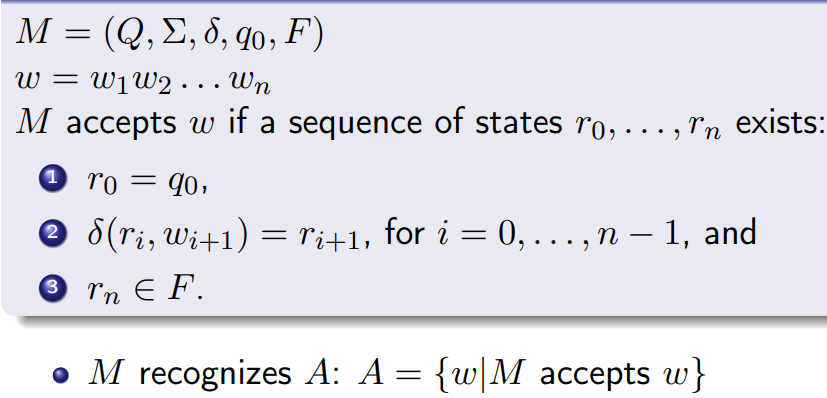
\includegraphics[scale=0.82]{solution/5-1.png}
    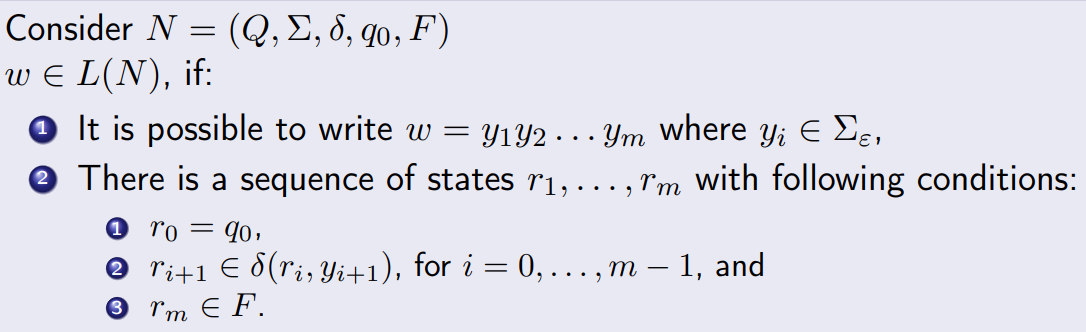
\includegraphics[scale=0.82]{solution/5-2.png}
    \includegraphics[scale=0.82]{solution/5-3.png}
\end{figure}

\begin{figure}[H]
    \centering
    \includegraphics[scale=0.82]{solution/5-4.png}
    \includegraphics[scale=0.82]{solution/5-5.png}
\end{figure}

همچنین از این 
\href{https://www.geeksforgeeks.org/3-coloring-is-np-complete/}{لینک} و
این 
\href{http://cs.bme.hu/thalg/3sat-to-3col.pdf}{لینک}
نیز کمک گرفته‌ایم. حال خودمان به طور مختصر شرح می‌دهیم :)).\\

زبان صوری:
\begin{center}
    \lr{L = $\{<G,k>\;|\;$ G is a graph of size n and $\exists c_1,\ldots,c_n\;\in\; \{1,\ldots,k\}$ such that 
    $\forall i,j\;\in\;1,\ldots,n\;: (v_i,v_j) \in E(G) \;
    \longrightarrow \; c_i \neq c_j\}$}
\end{center}

شرط نوشته شده همان Kرنگ پذیری در گراف است.
حال به اثبات می‌پردازیم:\\
یک verifire مانند v برای L میسازیم.

بدینگونه عمل میکند که به ازای هر یال در G چک میکند که رنگ 2 سر یال متفاوت باشند.
همچنین تعداد رنگ‌ها ماکسیمم برابر K باشد.
اگر n راس داشته باشیم،
$O(n^2)$ یال داریم که نتیجه میشود verifire، چندجمله‌ای است.

حال برای اینکه نشان دهیم این مسئله NP-complete است،
مسئله \lr{3-sat} را به آن کاهش می‌دهیم. این کار را به کاهش به زیرمجموعه‌ی سوالمان یعنی 
\lr{3 coloring} انجام میدهیم.

ابتدا یک مثلث با سه راس
\lr{T,F,B(true, false, base)} میسازیم. هر ست نشاندهنده لیبل ها برای 
vertices است.
از انجا که مثلث به 3 رنگ برای رنگ امیزی نیاز دارد، به 3 رنگ برای رنگ امیزی G نیاز داریم.
حال دو راس $v_i$ و $\Bar{v_i}$ اضافه میکنیم. 
( برای هر \lr{lateral} $x_i$ در مسئله 
$3-sat$ ).
حال برای هر $i$، یک مثلث با راس های
B, $v_i$, $\Bar{v_i}$ میسازیم. این کار باعث میشود رنگ متفاوتی با B داشته باشند.
شکل زیر را ببینید:
\begin{figure}[H]
    \centering
    \includegraphics[scale=1.2]{solution/5-6.png}
\end{figure}
حال به سراغ کلاز میرویم.
برای کلاز 
$C_i = a \vee b \vee c$ میخواهیم 
خروجی برابر T باشد اگر 
$C_i$ satisfied شده باشد و در غیر این صورت برابر F باشد.
شکل زیر را ببینید:
\begin{figure}[H]
    \centering
    \includegraphics{solution/5-7.png}
\end{figure}
نود $a \vee b$ خروجی 
$a \vee b$ را کپچر می‌کند و procedure یکسان برای 
$(a \vee b) \vee c$ تکرار می‌کنیم.

اگر تمامی انها به F شدند آنگاه نود خورجی نیز باید F باشد.
اگر یکی از انها T باشد یعنی یک رنگ امیزی درست وجود دارد پس خروجی نیز باید T باشد.
برای اطمینان اینکه خروجی ما رنگ امیزی درستی میدهد، از خروجی به F یک یال میکشیم تا نتواند F بشود.
\begin{figure}[H]
    \centering
    \includegraphics[scale=0.9]{solution/5-8.png}
\end{figure}

حال اگر مسئله $3-sat$، به نوعی 
satisfiable باشد،
اگر $x_i$ True باشد، ما $v_i$ را با T
و $\Bar{v_i}$ را با F رنگ میکنیم.

پس هر کلاز satisfiable است، بنابراین حداقل یکی از a، b، c برای هر عبارت True هستند، به این معنی که با توجه به ساختار ما، ابزار 3 رنگ می شود و گره خروجی به رنگ T است.
برای تکمیل کامل این قسمت به راه زیر که به عنوان سورس ذکر شد، توجه بفرمایید:
\begin{figure}[H]
    \centering
    \includegraphics[scale=0.92]{solution/5-9.png}
\end{figure}

\begin{figure}[H]
    \centering
    \includegraphics[scale=0.92]{solution/5-10.png}
\end{figure}

\begin{figure}[H]
    \centering
    \includegraphics[scale=0.92]{solution/5-11.png}
\end{figure}


\subsection*{2. }
این مسئله همان مسئله
\lr{exact-cover}
است.

زبان صوری:
\begin{center}
    \lr{L = $\{<S,\{S_1,\ldots,S_k\}>\; | \bigcup_{s\in\{S_1,\ldots,S_k\}}s = S$ and for some $J \subset \{1,\ldots,k\}$ we have $\cup_{j\in J}S_j = S,\;
    \forall i,j\;\in \; J: S_i \cap S_j = \emptyset\}$}
\end{center}
ابتدا نشان می‌دهیم مسئله NP است.
یک وریفایر چندجمله‌ای به عنوان certificate تعدادی اندیس ورودی میگیرد.
ابتدا چک میکند که اندیس بین 1 تا k باشند.
سپس روی هر $S_i$ حرکت میکند و هر عضوی را که از ان میبند، علامت میزند. اگر تمام اعضای S دقیقا یکبار علامت خورده باشند، ورودی را میپذیرد.
این عملیات چندجمله ای است بنابراین 
$L\in NP$.

برای NP-complete،
مسئله sat را به آن کاهش می‌دهیم.
ورودی $\sigma$ را به صورت 
\lr{conjuctive normal form}
برای sat در نظر میگیریم.
فرض کنید $\sigma$ شامل nتا متغیر 
$x_i$ و $l$ کلاز باشد.
کلاز
$c_j$ را به سورت زیر نمایش میدهیم:
\begin{center}
    $c_j = L_{j_1} \vee \ldots \vee L_{j_{m_j}}$
\end{center}
در این نمایش،
$m_j$ تعداد لیترالهای کلاز جی ام است.
حال S را به شکل زیر در نظر بگیرید:
\begin{center}
    $S = \{x_i\;|\; 1 \leq i \leq n\} \cup \{c_j\;|\;1\leq j\leq l\}\cup \{p_{jk}\;|\;1\leq j \leq l,\; 1 \leq k \leq m_j \}$
\end{center}
حال مجموعه $S_i$ها:
\begin{itemize}
    \item $\{p_{jk}\}$ \lr{for every} $p_{jk}$\\
    \item $T_i = \{x_i\} \cup \{p_{jk} | L_{jk} = \Bar{x_i}:$
    \lr{for every $x_i\}$}
    \item $F_i = \{x_i\} \cup \{p_{jk} | L_{jk} = x_i:$
    \lr{for every $x_i\}$}
    \item $\{c_j, p_{jk}\}$: \lr{for every} $c_j$ \lr{and every} $p_{jk}$
\end{itemize}
حال ادعا میکنیم که $\sigma$ به نوعی satisfiable است اگر و فقط اگر 
مجموعه $S$ با $S_i$های ساخته شده،
\lr{exact-cover} داشته باشد.
اگر satisfiable بود،
اگر 
$x_i = 1$ انگاه $T_i$ و در غیر این صورت،
$F_i$ را انتخاب میکنیم.
به ازای هر $c_j$ نیز یکی از مجموعه های 
$\{c_j,p_{jk}\}$ را برمیداریم که لیترال جایگاه kام آن برابر یک است.
اگر $T_i$ انتخاب شده باشد، تمام تکررهای صفرکننده $x_i$ نیز انتخاب شده است.
همین قضیه برای $F_i$ نیز برقرار است.
بنابراین با برداشتن $T_i$ها و $F_i$ها به شکل گفته شده،
$p_{jk}$های مربوط به  لیترالهای صفر انتخاب شده‌اند.
چونکه حداقل یک لیترال برابر 1 دارند هم تمام $c_j$ ها برداشته میشوند.
حال مجموعه های
$\{p_{jk}\}$
را طوری انتخاب میکنیم که هر
$p_{jk}$
نیز دقیقا یکبار تکرار شوند.بنابراین یک 
\lr{exact-cover} برای $S$ ساخته میشود.

حال اگر یک 
\lr{exact cover}
برای $S$ داشته باشیم؛
از بین هر 
$T_i$و $F_i$،
دقیقا یکی انتخاب شده است.
اگر 
$T_i$ انتخاب شده بود مقدار $x_i$ را یک و در غیر این صورت 0 میگذاریم.
برای هر کلاز $c_j$ نیز یکی از 
$\{c_j, p_{jk}\}$ها انتخاب شده است.
اگر 
$x_i = L_{jk}$
باشد، در این صورت 
$T_i$ انتخاب شده و $x_i$ برابر یک است. مشابه همین برای
$\Bar{x_i}$ برقرار است و اگر F انتخاب شده باشد، صفر میشود.
بنابراین تمام کلازها satisfy شده‌اند و $\sigma$ به نوعی satisfiable است.

بنابراین این زبان NP-complete است.

برای حل این سوال از یکی از بچه‌ها و همچنین به طور کامل از این 
\href{https://www.seas.upenn.edu/~cis5110/notes/cis511-sl15.pdf}{لینک}
و این 
\href{https://web.stanford.edu/class/archive/cs/cs103/cs103.1132/lectures/27/Small27.pdf}{لینک}
کمک گرفته شده است.

\begin{figure}[H]
    \centering
    \includegraphics[scale=0.95]{solution/5-12.png}
\end{figure}
\begin{figure}[H]
    \centering
    \includegraphics[scale=0.95]{solution/5-13.png}
\end{figure}
\begin{figure}[H]
    \centering
    \includegraphics[scale=0.95]{solution/5-14.png}
\end{figure}
\begin{figure}[H]
    \centering
    \includegraphics[scale=0.95]{solution/5-15.png}
\end{figure}
\begin{figure}[H]
    \centering
    \includegraphics[scale=0.95]{solution/5-16.png}
\end{figure}
\begin{figure}[H]
    \centering
    \includegraphics[scale=0.95]{solution/5-17.png}
\end{figure}

\subsection*{3. }
برای حل این سوال از این 
\href{https://www.cs.cornell.edu/courses/cs4820/2018fa/lectures/subset_sum.pdf}{لینک} کمک گرفته شده است.
همچنین ایده سوال از یکی از بچه های کلاس پرسیده شده است.

زبان صوری:
\begin{figure}[H]
    \centering
    \includegraphics[scale=0.75]{solution/5-18.png}
\end{figure}

ابتدا راه یکی از منابع را ببینیم:
\begin{figure}[H]
    \centering
    \includegraphics[scale=1.2]{solution/5-19.png}
\end{figure}
\begin{figure}[H]
    \centering
    \includegraphics[scale=1.2]{solution/5-20.png}
\end{figure}
\begin{figure}[H]
    \centering
    \includegraphics[scale=1.2]{solution/5-21.png}
\end{figure}

یک وریفایر چندجمله ای به عنوان سرتیفیکیت تعدادی اندیس ورودی میگیرد.
وریفایر ابتدا چک میکند که این اندیس ها بین 1 تا n باشند.
سپس اعضا را جمع زده و بررسی میکند که حاصل M شده است یا خیر.این کار در زمان چند جمله‌ای قابل انجام است و $L\in NP$.

حال مشئله $3-sat$ را به ان کاهش میدهیم.
مانند بخش قبل فرض میکنیم $\sigma$ یک ورودی از $3-sat$ با متغیرهای
$x_i$ و کلازهای
$c_j$ است.
به ازای هر $x_i$ 
2 عدد q و w را در نظر میگیریم.
به ازای هر کلاز هم 2 عدد
g و h را در نظر میگیریم.
فرض میکنیم l متغیر $x_i$ و همچنین
k متغیر $c_j$ داریم.
اعداد w و q در l رقم پرارزش خود دارای یک رقم یک و باقی رقم صفر هستند.
در واقع اعداد $w_i$ و $q_i$ در جایگاه i این مقدار را دارند.
رقم jام از  k
رقم کم ارزش اگر متغیر ما در $c_j$ امده باشد برابر یک و درغیر این صورت صفر هستند.
اعداد g و h نیز در k رقم کم ارزشتر تنها دارای یک در جایگاه i هستند.
مثال زیر را ببینید:
\begin{figure}[H]
    \centering
    \includegraphics[scale=1]{solution/5-22.png}
    \includegraphics[scale=0.8]{solution/5-23.png}
\end{figure}
ادعا میکنیم که ورودی $\sigma$ به نوعی satisfiable است اگرو تنها اگر مجموعه اعداد ساخته شده و مقدار t عضو زبان L باشد. دقت کنید 
y و z  در تصویر همان q و w گفته شده هستند.

\subsubsection*{طرف اول}
اگر satisfiable باششد،
زیرمجموعه از اعداد ورودی را به این شکل میسازیم:

اگر متغیر x برابر یک بود، $y_i$ و در غیر این صورت $z_i$ را انتخاب می‌کنیم.
اگر اعداد را جمع کنیم، عدد حاصل دارای یک رقم 1 در هر یک از lرقم پرارزشتر خود است.
همچنین هریک از kرقم کم ارزش ان بین 1 و 3 اسن زیرا هر کلاز 
satisfy شده است و بین یک تا سه  لیترال ان مقدار یک دارد.
در نتیجه از g و h ها تعداد مناسب را طوری  انتخاب میکنیم که جمع به t برسد.

\subsubsection*{طرف دوم}
حال اگر جمع برابر t باشد،
اگر این زیرمجموعه متغیر y داشت، مقدار متغیر متناظر x ان را یک میکنیم. در غیر این صورت 0 میگذاریم.
همچنین با توجه به جدول بالا از بین همه متغیرهای y و z دقیقا یکی انتخاب شده است متغیر x متناظر مقداردهی شده است.
چون جمع هر ستون برابر 3 هست، نتیجه میشود حتما یکی از لیترالهای مربوط به هر کلاز انتخاب شده و 1 شده است.
در نتیجه همه کلازها satisfy شده و $\sigma$ نیز satisfiable است.

بنابراین اثبات شد. 

حل این سوال از سیپسر برداشته شده است.:

\begin{figure}[H]
    \centering
    \includegraphics[scale=1.1]{solution/r1.png}
\end{figure}
\begin{figure}[H]
    \centering
    \includegraphics[scale=1.1]{solution/r2.png}
\end{figure}
\begin{figure}[H]
    \centering
    \includegraphics[scale=1.1]{solution/r3.png}
\end{figure}

در هر 3 بخش، راه حداقل یک سورس به همراه توضیحات بنده وجود دارد تا نقصانی وجود نداشته باشد.